% Created by tikzDevice version 0.10.1 on 2016-08-25 15:50:23
% !TEX encoding = UTF-8 Unicode
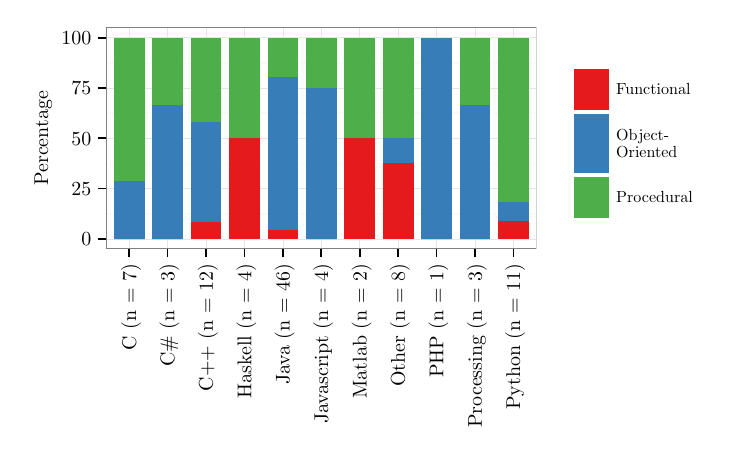
\begin{tikzpicture}[x=1pt,y=1pt]
\definecolor{fillColor}{RGB}{255,255,255}
\path[use as bounding box,fill=fillColor,fill opacity=0.00] (0,0) rectangle (252.94,144.54);
\begin{scope}
\path[clip] (  0.00,  0.00) rectangle (252.94,144.54);
\definecolor{drawColor}{RGB}{255,255,255}
\definecolor{fillColor}{RGB}{255,255,255}

\path[draw=drawColor,line width= 0.6pt,line join=round,line cap=round,fill=fillColor] (  0.00,  0.00) rectangle (252.94,144.54);
\end{scope}
\begin{scope}
\path[clip] ( 28.36, 64.59) rectangle (183.84,144.54);
\definecolor{fillColor}{RGB}{255,255,255}

\path[fill=fillColor] ( 28.36, 64.59) rectangle (183.84,144.54);
\definecolor{drawColor}{gray}{0.98}

\path[draw=drawColor,line width= 0.6pt,line join=round] ( 28.36, 77.31) --
	(183.84, 77.31);

\path[draw=drawColor,line width= 0.6pt,line join=round] ( 28.36, 95.48) --
	(183.84, 95.48);

\path[draw=drawColor,line width= 0.6pt,line join=round] ( 28.36,113.65) --
	(183.84,113.65);

\path[draw=drawColor,line width= 0.6pt,line join=round] ( 28.36,131.82) --
	(183.84,131.82);
\definecolor{drawColor}{gray}{0.90}

\path[draw=drawColor,line width= 0.2pt,line join=round] ( 28.36, 68.22) --
	(183.84, 68.22);

\path[draw=drawColor,line width= 0.2pt,line join=round] ( 28.36, 86.39) --
	(183.84, 86.39);

\path[draw=drawColor,line width= 0.2pt,line join=round] ( 28.36,104.56) --
	(183.84,104.56);

\path[draw=drawColor,line width= 0.2pt,line join=round] ( 28.36,122.73) --
	(183.84,122.73);

\path[draw=drawColor,line width= 0.2pt,line join=round] ( 28.36,140.91) --
	(183.84,140.91);

\path[draw=drawColor,line width= 0.2pt,line join=round] ( 36.69, 64.59) --
	( 36.69,144.54);

\path[draw=drawColor,line width= 0.2pt,line join=round] ( 50.57, 64.59) --
	( 50.57,144.54);

\path[draw=drawColor,line width= 0.2pt,line join=round] ( 64.45, 64.59) --
	( 64.45,144.54);

\path[draw=drawColor,line width= 0.2pt,line join=round] ( 78.33, 64.59) --
	( 78.33,144.54);

\path[draw=drawColor,line width= 0.2pt,line join=round] ( 92.22, 64.59) --
	( 92.22,144.54);

\path[draw=drawColor,line width= 0.2pt,line join=round] (106.10, 64.59) --
	(106.10,144.54);

\path[draw=drawColor,line width= 0.2pt,line join=round] (119.98, 64.59) --
	(119.98,144.54);

\path[draw=drawColor,line width= 0.2pt,line join=round] (133.86, 64.59) --
	(133.86,144.54);

\path[draw=drawColor,line width= 0.2pt,line join=round] (147.74, 64.59) --
	(147.74,144.54);

\path[draw=drawColor,line width= 0.2pt,line join=round] (161.63, 64.59) --
	(161.63,144.54);

\path[draw=drawColor,line width= 0.2pt,line join=round] (175.51, 64.59) --
	(175.51,144.54);
\definecolor{fillColor}{RGB}{228,26,28}

\path[fill=fillColor] ( 31.13, 68.22) rectangle ( 42.24, 68.22);
\definecolor{fillColor}{RGB}{55,126,184}

\path[fill=fillColor] ( 31.13, 68.22) rectangle ( 42.24, 88.99);
\definecolor{fillColor}{RGB}{77,175,74}

\path[fill=fillColor] ( 31.13, 88.99) rectangle ( 42.24,140.91);
\definecolor{fillColor}{RGB}{228,26,28}

\path[fill=fillColor] ( 45.02, 68.22) rectangle ( 56.12, 68.22);
\definecolor{fillColor}{RGB}{55,126,184}

\path[fill=fillColor] ( 45.02, 68.22) rectangle ( 56.12,116.68);
\definecolor{fillColor}{RGB}{77,175,74}

\path[fill=fillColor] ( 45.02,116.68) rectangle ( 56.12,140.91);
\definecolor{fillColor}{RGB}{228,26,28}

\path[fill=fillColor] ( 58.90, 68.22) rectangle ( 70.00, 74.28);
\definecolor{fillColor}{RGB}{55,126,184}

\path[fill=fillColor] ( 58.90, 74.28) rectangle ( 70.00,110.62);
\definecolor{fillColor}{RGB}{77,175,74}

\path[fill=fillColor] ( 58.90,110.62) rectangle ( 70.00,140.91);
\definecolor{fillColor}{RGB}{228,26,28}

\path[fill=fillColor] ( 72.78, 68.22) rectangle ( 83.89,104.56);
\definecolor{fillColor}{RGB}{55,126,184}

\path[fill=fillColor] ( 72.78,104.56) rectangle ( 83.89,104.56);
\definecolor{fillColor}{RGB}{77,175,74}

\path[fill=fillColor] ( 72.78,104.56) rectangle ( 83.89,140.91);
\definecolor{fillColor}{RGB}{228,26,28}

\path[fill=fillColor] ( 86.66, 68.22) rectangle ( 97.77, 71.38);
\definecolor{fillColor}{RGB}{55,126,184}

\path[fill=fillColor] ( 86.66, 71.38) rectangle ( 97.77,126.68);
\definecolor{fillColor}{RGB}{77,175,74}

\path[fill=fillColor] ( 86.66,126.68) rectangle ( 97.77,140.91);
\definecolor{fillColor}{RGB}{228,26,28}

\path[fill=fillColor] (100.54, 68.22) rectangle (111.65, 68.22);
\definecolor{fillColor}{RGB}{55,126,184}

\path[fill=fillColor] (100.54, 68.22) rectangle (111.65,122.73);
\definecolor{fillColor}{RGB}{77,175,74}

\path[fill=fillColor] (100.54,122.73) rectangle (111.65,140.91);
\definecolor{fillColor}{RGB}{228,26,28}

\path[fill=fillColor] (114.43, 68.22) rectangle (125.53,104.56);
\definecolor{fillColor}{RGB}{55,126,184}

\path[fill=fillColor] (114.43,104.56) rectangle (125.53,104.56);
\definecolor{fillColor}{RGB}{77,175,74}

\path[fill=fillColor] (114.43,104.56) rectangle (125.53,140.91);
\definecolor{fillColor}{RGB}{228,26,28}

\path[fill=fillColor] (128.31, 68.22) rectangle (139.42, 95.48);
\definecolor{fillColor}{RGB}{55,126,184}

\path[fill=fillColor] (128.31, 95.48) rectangle (139.42,104.56);
\definecolor{fillColor}{RGB}{77,175,74}

\path[fill=fillColor] (128.31,104.56) rectangle (139.42,140.91);
\definecolor{fillColor}{RGB}{228,26,28}

\path[fill=fillColor] (142.19, 68.22) rectangle (153.30, 68.22);
\definecolor{fillColor}{RGB}{55,126,184}

\path[fill=fillColor] (142.19, 68.22) rectangle (153.30,140.91);
\definecolor{fillColor}{RGB}{77,175,74}

\path[fill=fillColor] (142.19,140.91) rectangle (153.30,140.91);
\definecolor{fillColor}{RGB}{228,26,28}

\path[fill=fillColor] (156.07, 68.22) rectangle (167.18, 68.22);
\definecolor{fillColor}{RGB}{55,126,184}

\path[fill=fillColor] (156.07, 68.22) rectangle (167.18,116.68);
\definecolor{fillColor}{RGB}{77,175,74}

\path[fill=fillColor] (156.07,116.68) rectangle (167.18,140.91);
\definecolor{fillColor}{RGB}{228,26,28}

\path[fill=fillColor] (169.96, 68.22) rectangle (181.06, 74.83);
\definecolor{fillColor}{RGB}{55,126,184}

\path[fill=fillColor] (169.96, 74.83) rectangle (181.06, 81.44);
\definecolor{fillColor}{RGB}{77,175,74}

\path[fill=fillColor] (169.96, 81.44) rectangle (181.06,140.91);
\definecolor{drawColor}{gray}{0.50}

\path[draw=drawColor,line width= 0.6pt,line join=round,line cap=round] ( 28.36, 64.59) rectangle (183.84,144.54);
\end{scope}
\begin{scope}
\path[clip] (  0.00,  0.00) rectangle (252.94,144.54);
\definecolor{drawColor}{RGB}{0,0,0}

\node[text=drawColor,anchor=base east,inner sep=0pt, outer sep=0pt, scale=  0.72] at ( 22.96, 65.74) {0};

\node[text=drawColor,anchor=base east,inner sep=0pt, outer sep=0pt, scale=  0.72] at ( 22.96, 83.91) {25};

\node[text=drawColor,anchor=base east,inner sep=0pt, outer sep=0pt, scale=  0.72] at ( 22.96,102.08) {50};

\node[text=drawColor,anchor=base east,inner sep=0pt, outer sep=0pt, scale=  0.72] at ( 22.96,120.25) {75};

\node[text=drawColor,anchor=base east,inner sep=0pt, outer sep=0pt, scale=  0.72] at ( 22.96,138.43) {100};
\end{scope}
\begin{scope}
\path[clip] (  0.00,  0.00) rectangle (252.94,144.54);
\definecolor{drawColor}{RGB}{0,0,0}

\path[draw=drawColor,line width= 0.6pt,line join=round] ( 25.36, 68.22) --
	( 28.36, 68.22);

\path[draw=drawColor,line width= 0.6pt,line join=round] ( 25.36, 86.39) --
	( 28.36, 86.39);

\path[draw=drawColor,line width= 0.6pt,line join=round] ( 25.36,104.56) --
	( 28.36,104.56);

\path[draw=drawColor,line width= 0.6pt,line join=round] ( 25.36,122.73) --
	( 28.36,122.73);

\path[draw=drawColor,line width= 0.6pt,line join=round] ( 25.36,140.91) --
	( 28.36,140.91);
\end{scope}
\begin{scope}
\path[clip] (  0.00,  0.00) rectangle (252.94,144.54);
\definecolor{drawColor}{RGB}{0,0,0}

\path[draw=drawColor,line width= 0.6pt,line join=round] ( 36.69, 61.59) --
	( 36.69, 64.59);

\path[draw=drawColor,line width= 0.6pt,line join=round] ( 50.57, 61.59) --
	( 50.57, 64.59);

\path[draw=drawColor,line width= 0.6pt,line join=round] ( 64.45, 61.59) --
	( 64.45, 64.59);

\path[draw=drawColor,line width= 0.6pt,line join=round] ( 78.33, 61.59) --
	( 78.33, 64.59);

\path[draw=drawColor,line width= 0.6pt,line join=round] ( 92.22, 61.59) --
	( 92.22, 64.59);

\path[draw=drawColor,line width= 0.6pt,line join=round] (106.10, 61.59) --
	(106.10, 64.59);

\path[draw=drawColor,line width= 0.6pt,line join=round] (119.98, 61.59) --
	(119.98, 64.59);

\path[draw=drawColor,line width= 0.6pt,line join=round] (133.86, 61.59) --
	(133.86, 64.59);

\path[draw=drawColor,line width= 0.6pt,line join=round] (147.74, 61.59) --
	(147.74, 64.59);

\path[draw=drawColor,line width= 0.6pt,line join=round] (161.63, 61.59) --
	(161.63, 64.59);

\path[draw=drawColor,line width= 0.6pt,line join=round] (175.51, 61.59) --
	(175.51, 64.59);
\end{scope}
\begin{scope}
\path[clip] (  0.00,  0.00) rectangle (252.94,144.54);
\definecolor{drawColor}{RGB}{0,0,0}

\node[text=drawColor,rotate= 90.00,anchor=base east,inner sep=0pt, outer sep=0pt, scale=  0.72] at ( 39.16, 59.19) {C (n = 7)};

\node[text=drawColor,rotate= 90.00,anchor=base east,inner sep=0pt, outer sep=0pt, scale=  0.72] at ( 53.05, 59.19) {C\# (n = 3)};

\node[text=drawColor,rotate= 90.00,anchor=base east,inner sep=0pt, outer sep=0pt, scale=  0.72] at ( 66.93, 59.19) {C++ (n = 12)};

\node[text=drawColor,rotate= 90.00,anchor=base east,inner sep=0pt, outer sep=0pt, scale=  0.72] at ( 80.81, 59.19) {Haskell (n = 4)};

\node[text=drawColor,rotate= 90.00,anchor=base east,inner sep=0pt, outer sep=0pt, scale=  0.72] at ( 94.69, 59.19) {Java (n = 46)};

\node[text=drawColor,rotate= 90.00,anchor=base east,inner sep=0pt, outer sep=0pt, scale=  0.72] at (108.58, 59.19) {Javascript (n = 4)};

\node[text=drawColor,rotate= 90.00,anchor=base east,inner sep=0pt, outer sep=0pt, scale=  0.72] at (122.46, 59.19) {Matlab (n = 2)};

\node[text=drawColor,rotate= 90.00,anchor=base east,inner sep=0pt, outer sep=0pt, scale=  0.72] at (136.34, 59.19) {Other (n = 8)};

\node[text=drawColor,rotate= 90.00,anchor=base east,inner sep=0pt, outer sep=0pt, scale=  0.72] at (150.22, 59.19) {PHP (n = 1)};

\node[text=drawColor,rotate= 90.00,anchor=base east,inner sep=0pt, outer sep=0pt, scale=  0.72] at (164.11, 59.19) {Processing (n = 3)};

\node[text=drawColor,rotate= 90.00,anchor=base east,inner sep=0pt, outer sep=0pt, scale=  0.72] at (177.99, 59.19) {Python (n = 11)};
\end{scope}
\begin{scope}
\path[clip] (  0.00,  0.00) rectangle (252.94,144.54);
\definecolor{drawColor}{RGB}{0,0,0}

\node[text=drawColor,rotate= 90.00,anchor=base,inner sep=0pt, outer sep=0pt, scale=  0.72] at (  7.36,104.56) {Percentage};
\end{scope}
\begin{scope}
\path[clip] (  0.00,  0.00) rectangle (252.94,144.54);
\definecolor{fillColor}{RGB}{255,255,255}

\path[fill=fillColor] (192.37, 70.76) rectangle (244.41,138.36);
\end{scope}
\begin{scope}
\path[clip] (  0.00,  0.00) rectangle (252.94,144.54);
\definecolor{fillColor}{RGB}{228,26,28}

\path[fill=fillColor] (197.35,114.78) rectangle (210.16,129.77);
\end{scope}
\begin{scope}
\path[clip] (  0.00,  0.00) rectangle (252.94,144.54);
\definecolor{fillColor}{RGB}{55,126,184}

\path[fill=fillColor] (197.35, 92.15) rectangle (210.16,113.36);
\end{scope}
\begin{scope}
\path[clip] (  0.00,  0.00) rectangle (252.94,144.54);
\definecolor{fillColor}{RGB}{77,175,74}

\path[fill=fillColor] (197.35, 75.74) rectangle (210.16, 90.73);
\end{scope}
\begin{scope}
\path[clip] (  0.00,  0.00) rectangle (252.94,144.54);
\definecolor{drawColor}{RGB}{0,0,0}

\node[text=drawColor,anchor=base west,inner sep=0pt, outer sep=0pt, scale=  0.58] at (212.68,126.51) {};

\node[text=drawColor,anchor=base west,inner sep=0pt, outer sep=0pt, scale=  0.58] at (212.68,120.29) {Functional};

\node[text=drawColor,anchor=base west,inner sep=0pt, outer sep=0pt, scale=  0.58] at (212.68,114.07) {};
\end{scope}
\begin{scope}
\path[clip] (  0.00,  0.00) rectangle (252.94,144.54);
\definecolor{drawColor}{RGB}{0,0,0}

\node[text=drawColor,anchor=base west,inner sep=0pt, outer sep=0pt, scale=  0.58] at (212.68,110.10) {};

\node[text=drawColor,anchor=base west,inner sep=0pt, outer sep=0pt, scale=  0.58] at (212.68,103.88) {Object-};

\node[text=drawColor,anchor=base west,inner sep=0pt, outer sep=0pt, scale=  0.58] at (212.68, 97.66) {Oriented};

\node[text=drawColor,anchor=base west,inner sep=0pt, outer sep=0pt, scale=  0.58] at (212.68, 91.44) {};
\end{scope}
\begin{scope}
\path[clip] (  0.00,  0.00) rectangle (252.94,144.54);
\definecolor{drawColor}{RGB}{0,0,0}

\node[text=drawColor,anchor=base west,inner sep=0pt, outer sep=0pt, scale=  0.58] at (212.68, 87.47) {};

\node[text=drawColor,anchor=base west,inner sep=0pt, outer sep=0pt, scale=  0.58] at (212.68, 81.25) {Procedural};

\node[text=drawColor,anchor=base west,inner sep=0pt, outer sep=0pt, scale=  0.58] at (212.68, 75.03) {};
\end{scope}
\end{tikzpicture}
